\chapter{Oscillation of neutral $B$-mesons}

The phenomenon of neutral mesons transforming into their respective antiparticle was first investigated by Gell-Main and Pais in 1955 \cite{PhysRev.97.1387}.
The CKM-matrix was introduced as an extension of the Cabbibo matrix in 1973 after discovering $CP$ violation which could not be explained with 4-quark-mixing \cite{10.1143/PTP.49.652}.
Each element of the matrix describes a transition between quark generations.
The neutral B meson $B^0_d(d\bar b)$ or respectively $B^0_s(s\bar d)$ can oscillate via two components, the on-shell $(E^2= p^2+m^2)$ and off-shell $(E^2\neq p^2+m^2)$ components which are shown in \ref{fig:feynmanOnshell} and \ref{fig:feynmanOffshell} respectively.
\begin{figure}
    \centering
    \begin{subfigure}[B]{.5\textwidth}   % 1st subfigure
        \centering
        \includegraphics[width=.8\textwidth]{figs/feynmanOnshell.png}
        \caption{On-shell contribution.}
        \label{fig:feynmanOnshell}
    \end{subfigure}
    \begin{subfigure}[B]{.45\textwidth}   % 2nd subfigure
        \centering
        \includegraphics[width=.8\textwidth]{figs/feynmanOffshell.png}
        \caption{Off-shell contribution.}
        \label{fig:feynmanOffshell}
    \end{subfigure}
    \caption{Feynman diagram showing the neutral B meson oscillation \cite{Kpopp}.}
    \label{fig:feynmanDiagram}
\end{figure}
Measuring the oscillation frequency yields precise measurements of $V_{q_u b}$ and $V_{q_u d/s}$.
A time evolution can be deduced by introducing a mixing matrix in which non-diagonal elements occur due to oscillations via the box diagram \ref{fig:feynmanOnshell} and the on-shell contributions.
By diagonalising the mixing matrix an expression for the time evolution of flavour eigenstates can be found.
% Due to the on-shell contributions being much smaller than the off-shell contributions the oscillation frequency which results from a mass difference $\upDelta m_{d/s}$ is directly proportional to the matrix element $|V_{td}|^2$ resulting in an expression for the oscillation frequency
An expression for the oscillation frequency can be found due to the on-shell contribution being much smaller than the off-shell contributions $(\Gamma_{ij}<M_{ij})$ with $\upDelta m_{d/s}\propto |V_{td}|^2$ with $\upDelta m_{d/s}$ describing a mass difference \cite{artuso2019cp}.
The $B_d^0$ oscillation was first discovered at the ARGUS detector at DESY in 1987 \cite{ALBRECHT1987245}.
Earlier measurements were done by CLEO \cite{PhysRevLett.58.183}, MARK II \cite{SCHAAD1985188} and UA1 \cite{ALBAJAR1987247} collaborations.
Collisions of $e^+e^-$ at an energy of the $\Upsilon(4S)$ resonance produced $B^0_dB^0_d$ pairs which were used to measure the oscillation.
% Three analysis methods were used.
One of the methods was to search for a fully reconstructed decay of $\Upsilon(4S)\rightarrow B^0_dB^0_d /\bar B^0_d\bar B^0_d$ which decayed flavourspecific via $B_d^0\rightarrow D^{*-}\pi^+/D^{*-}l^+\nu$ and  $\bar B_d^0\rightarrow D^{*+}\pi^-/D^{*+}l^-\nu$.
A different method was to reconstruct one $B_d^0$ from the $\Upsilon(4S)$ and tag the other $B_d^0$ with a lepton.
Using the same decay channels for the reconstruction of $B_d^0$ makes this method less sensitive to background originating from lepton misidentification.
It yielded a time-integrated oscillation parameter $r= \frac{\mathcal{BR}(B\rightarrow \bar B\rightarrow \bar X)}{\mathcal{BR}(B\rightarrow X)}$ of $r=\num{0.21(0.08)}$ which meant for the matrix element $V_{td}\neq 0$ \cite{ALBRECHT1987245}.

\begin{wrapfigure}{l}{5cm}
    \centering
    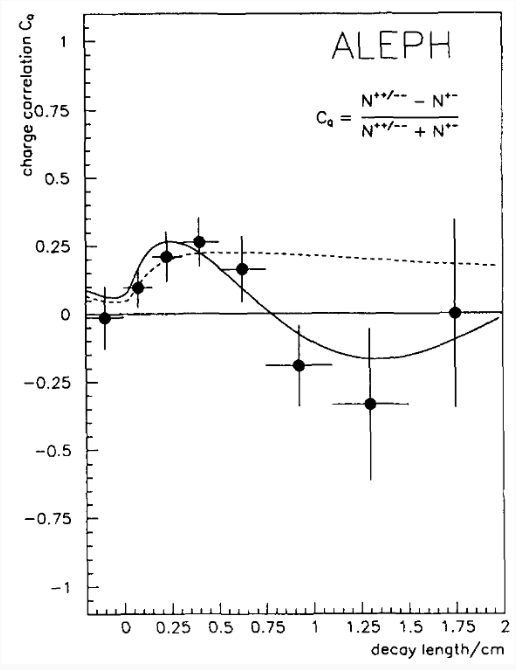
\includegraphics[width=0.3\textwidth]{figs/ALEPHresults.png}
    \caption{Fit to $Q_C(t)$ with a time dependent oscillation in data (solid) and a time independent approach (dashed) \cite{1993498}.}
    \label{fig:ALEPHresults}
\end{wrapfigure}
The ALEPH experiment at LEP measured the oscillation frequency $\upDelta m_d$ by tagging the state of $B_d^0$ at the time of production which decays semileptonic and at the time of decay which decays flavourspecific via $B_d^0\rightarrow D^{*-}X$ and $\bar B_d^0\rightarrow D^{*+}X$ \cite{1993498}.
Every \textit{correct} sign in the decay was defined as an unmixed event and vice versa by which a charge correlation function $C_Q(t)$ was defined.
At ALEPH the $B_d^0$ momentum was not reconstructed and the decay time was not calculated and only the decay length was used with boosting of $B_d^0$ that involved the momentum spectra.
Figure \ref{fig:ALEPHresults} shows an unbinned maximum likelihood fit to the decay length distribution to get $C_Q(t)$.
The involvement of the decay length distribution with the momentum spectra yielded the decay time.
An oscillation frequency of $\upDelta m_d = 0.52^{+0.10}_{-0.11}(\text{stat})^{+0.04}_{-0.05}(\text{syst})\, \text{ps}^{-1}$ was found \cite{1993498}.

\begin{wrapfigure}{l}{6.8cm}
    \centering
    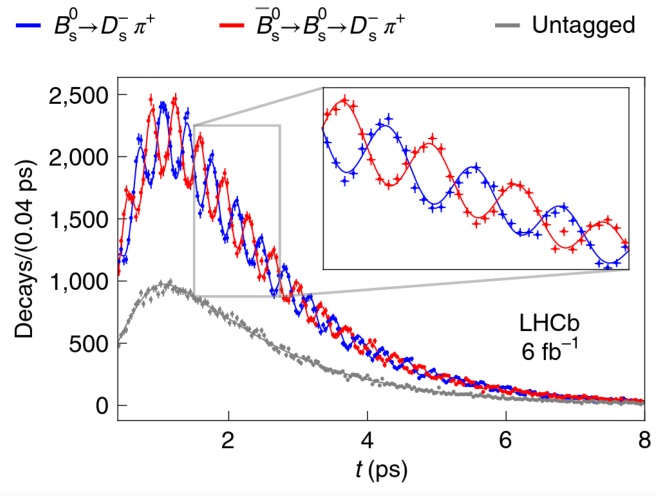
\includegraphics[width=0.5\textwidth]{figs/LHCbResults.png}
    \caption{Measurement of $B_s^0$ oscillations with the LHCb experiment \cite{LHCb2}.}
    \label{fig:LHCbResults}
\end{wrapfigure}
The oscillation of $B_s^0$ is more likely than the $B_d^0$ oscillation, due to $|V_{ts}|>|V_{td}|$ and was first discovered at CDF II in 2006 \cite{PhysRevLett.97.242003}.
Due to the mass difference of $s$ quarks being larger than those of $d$ quarks, a better time resolution was needed.
Measurements of $\upDelta m_d$ with the LHCb experiment at the LHC could increase the precision in 2016 \cite{LHCb1} to a value of $\upDelta m_d = 0.505\pm0.0021\,(\text{stat})\pm0.001\,(\text{syst})\,\text{ps}^{-1}$ leading to a matrix element of $V_{td}=\num{8.6(0.2)e-3}$ \cite{Workman:2022ynf}.
A study from 2022 found an oscillation frequency for $B_s^0$ of $\upDelta m_s = 17.7683 \pm 0.0051\,(\text{stat}) \pm 0.0032\,(\text{syst})\,\text{ps}^{-1}$ \cite{LHCb2} which lead to a value for the matrix element of $V_{ts}=\num{41.5(0.9)e-3}$ \cite{Workman:2022ynf}.
In figure \ref{fig:LHCbResults} the measurements of $B_s^0$ oscillations from the LHCb experiment are shown.
Figure \ref{fig:LHCbResults} shows the decay time of the $B_s^0\rightarrow D_s^-\pi^+$ signal decays are shown with the unmixed components shown in blue and the mixed components shown in red.